\chapter{Проектирование}

\section{Моделирование прямого цифрового синтеза}

Смоделируем алгоритм метода прямого цифрового синтеза на языке Си для дальнейшей реализации на микроконтроллере.

\begin{code}
\captionof{listing}{Метод DDS.}
\begin{minted}[mathescape,linenos,frame=lines,breaklines]{text}
int main() {
  uint16_t p_acc, p_step;
  uint8_t addr = 0; // адрес ячейки

  p_acc = 0;    // аккумулятор фазы
  p_step = 128; // код частоты

  while(1)
  {
    addr = p_acc >> 8; // выделение старшей части аккумулятора фазы
    p_acc += p_step;   // шаг
    printf("%d 0x%X\n", addr, sinus[addr]); // вывод отсчёта
  }

  return 0;
}
\end{minted}
\end{code}

	Алгоритм программы представлен следующей блок-схемой.
	
\begin{figure}[H]
    \centering
    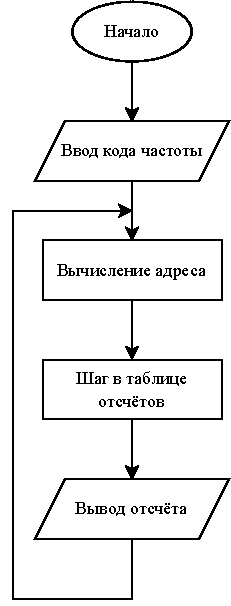
\includegraphics[width=0.45\textwidth]{../image/dds_block.pdf}
    \caption{Алгоритм метода DDS.}
\end{figure}
	
	Код частоты задаёт выходную частоту генератора. При значении 256 вывод будет следующий:
	
\begin{figure}[H]
    \centering
    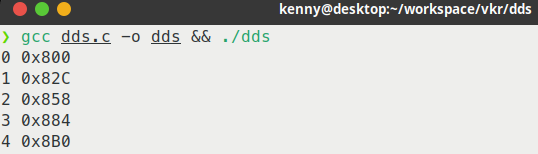
\includegraphics[width=0.6\textwidth]{../image/dds256.png}
    \caption{Формирование отсчётов при коде частоты 256.}
\end{figure}
	
	Увеличим код частоты в два раза и получим следующее:

\begin{figure}[H]
    \centering
    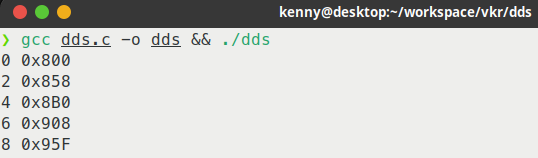
\includegraphics[width=0.6\textwidth]{../image/dds512.png}
    \caption{Формирование отсчётов при коде частоты 512.}
\end{figure}

	Как можно заметить отсчёты стали формироваться через один, соответственно частота вырастит в два раза. Теперь уменьшим частоту в два раза выставив код частоты 128.

\begin{figure}[H]
    \centering
    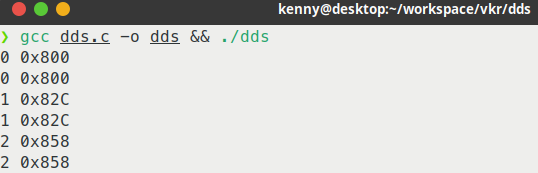
\includegraphics[width=0.6\textwidth]{../image/dds128.png}
    \caption{Формирование отсчётов при коде частоты 128.}
\end{figure}

	Программа стала выводить каждый отсчёт по два раза тем самым, понизив частоту.
	
	В данном виде модуляции код частоты просто абстрактное число, которое добавляется к аккумулятору фазы и узнать реальную частоту проблематично. Результат синтеза будет проверен опытным путём на микроконтроллере.

\section{Алгоритм работы}


\section{Схема генератора}
\begin{figure}[h]
    \centering
    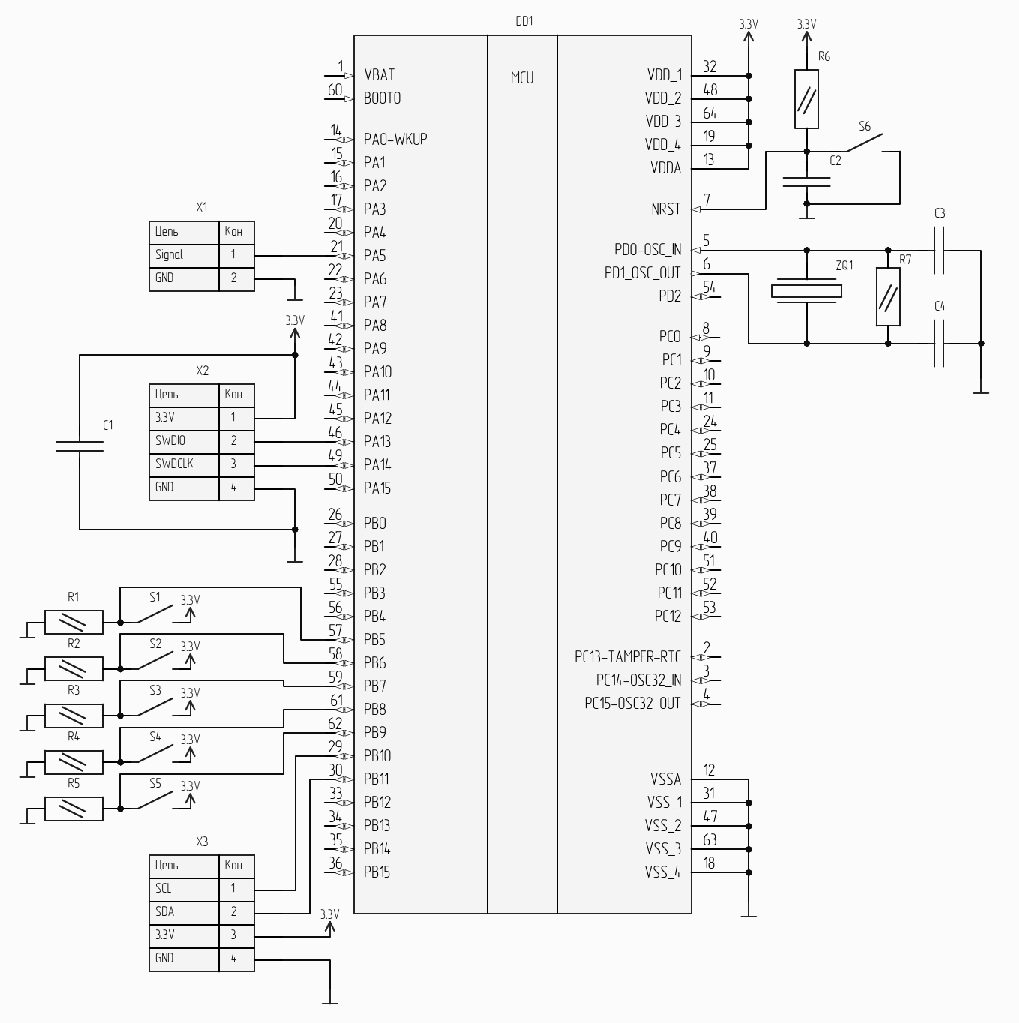
\includegraphics[width=1.0\textwidth]{../image/scheme-cropped.pdf}
    \caption{Схема электрическая принципиальная.}
\end{figure}

